\documentclass{hitec}
\author{AVL - rkerr2, jkoehle2, mfhoffm2, dcsimps2, roque2, srghnth2, mhaskar2}
\title{Avalon Online}
\usepackage{blindtext}
\usepackage{graphicx}
\usepackage{longtable}
\begin{document}
\maketitle

\settextfraction{0.9}

\tableofcontents

\section{Project Description and Process}
\subsection{The Project}
Our group has worked to create an online, playable version of the Avalon expansion to the popular board game Resistance. Avalon is a five to ten player, hidden roles game where the goal is for an informed minority to stop an uninformed majority from completing three missions successfully. Players are able to vote on teams to go on the missions and the players on the chosen teams select whether to pass or fail the missions. Our version also allows players to view information about previous votes and missions.

Since our game is meant to be played online, it removes some methods of gaining information from the standard game, such as facial expressions and body language. However, players gain the benefits of perfect memory since they can view records of previous votes, missions, and chat messages. Our main motivation for creating an online version of this game is to provide an easy way for people to play together, since it is often difficult to get a large enough group together in person.

\subsection{Development Process}
Since everyone in the team had taken computer science 427 last semester, we decided to start with the XP process described there as a base. Overall, everyone was relatively happy with the process as it was laid out, with only minor changes. The main objection everyone had to XP was test-driven development. The team agreed that requiring all tests to be written before any code ensures that classes are more thought out and better planned. However, the team disliked that you could not play with the code until you found the best way to tackle the problem, feeling that it stifled creativity too much. Therefore, as a group, we decided that our process would allow writing classes and functions first, as long as the tests are written immediately afterwards.

In terms of collaborative development, we used pair programming.  The extent to which a pair followed strict pair programming practices was left to the judgement of the pair, because forcing an incompatible pair to work together can be worse than not pairing at all.  But for the vast majority of the time, we followed the practice as usual. 
     
Our iterative development policy was standard Extreme Programming, with two-week iterations and weekly team meetings.  We found that scheduling went very smoothly.  Our meetings focused on discussing our progress and collaborating on parts of the code.  We also debated refactorings that needed to be done, or that we were in the process of doing.
\section{Requirements and Specification}
\subsection{Use Cases}

\begin{longtable}{l|l| p{6cm}}
\textbf{UC\#} & \textbf{Name}                 & \textbf{Description}                                                                                     \\
\hline
UC1           & Select Options, Start Game    & User can select game settings and create a game with those settings.                                     \\
UC2           & Select Server Info            & User can enter a server address and port number and be connected to the correct game.                    \\
UC3           & Assign Own Name               & User can enter a name to represent them during the game.                                                 \\
UC4           & Create Server                 & Startup client can create a server.                                                                      \\
UC5           & Join Game                     & Startup client can join a created game.                                                                  \\
UC6           & Propose Team                  & Player can propose a team for the mission if they are the leader.                                        \\
UC7           & Display Proposed Team         & Game client can display the proposed team for the players.                                               \\
UC8           & Display Leader                & Game client can display the leader for the players.                                                      \\
UC9           & Approve/Reject Team           & Players can vote to approve or reject the proposed team.                                                 \\
UC10          & Display Vote Progress         & Game client can display who has voted on the proposed team to the players.                               \\
UC11          & Display Team Vote Results     & Game client can display the results of a vote on a proposed team.                                        \\
UC12          & Accept Vote Results           & Players can accept the vote results.                                                                     \\
UC13          & Pass/Fail Mission             & Players can choose to either Pass or Fail the current mission if they are on the quest team.             \\
UC14          & Display Mission Vote Progress & Game client can display who has voted on the mission to the players.                                     \\
UC15          & Display Mission Results       & Game client can display the results of a mission to the players.                                         \\
UC16          & Accept Mission Results        & Players can accept the mission results.                                                                  \\
UC17          & Send Team Selection           & Game client can send the chosen team to the server.                                                      \\
UC18          & Confirm Team Selection        & Game client can confirm the chosen team with the server.                                                 \\
UC19          & Send Leader                   & Game client can send who the leader is to the server.                                                    \\
UC20          & Send Team Votes               & Game client can send players' votes on the proposed team to the server.                                  \\
UC21          & Send Team Vote Progress       & Server can send the game client who has voted on the proposed team.                                      \\
UC22          & Send Team Vote Results        & Server can send the game client the results of a vote on a proposed team.                                \\
UC23          & Send Mission Votes            & Game client can send players' votes on the current mission to the server.                                \\
UC24          & Send Mission Vote Progress    & Server can send the game client who has voted on the current mission.                                    \\
UC25          & Send Mission Vote Results     & Server can send the game client the results of a vote on the current mission.                            \\
UC26          & Input Chat Message            & Player can enter a message in the chat (and send it to the game client).                                 \\
UC27          & Display Chat                  & Game client can display updated chat to players.                                                         \\
UC28          & Send Chat Message             & Game client can send chat messages to the server.                                                        \\
UC29          & Propagate Chat Message        & Server can propagate chat messages to all game clients.                                                  \\
UC30          & Close Program                 & Players can close the program.                                                                           \\
UC31          & Drop From Server              & Game client can disconnect from the server.                                                              \\
UC32          & Die                           & Server can gently shut down game clients.                                                                \\
UC33          & Transition State              & Game client and server can communicate a state transition.                                               \\
UC34          & Transition to Game            & Startup client can transition to the game client.                                                        \\
UC35          & Reveal Roles                  & Game client can reveal every player's role to every player at the end of the game.                       \\
UC36          & Make Assassin Decision        & Player can choose who to assassinate if they are the Assassin.                                           \\
UC37          & Display Win/Loss              & Game client can tell player if they have won or lost.                                                    \\
UC38          & Dismiss Game                  & Player can dismiss the game.                                                                             \\
UC39          & Send Roles                    & Server can send roles to the game client.                                                                \\
UC40          & Send Assassin Decision        & Game client can send the assassin's decision to the server.                                              \\
UC41          & Send Win/Loss                 & Server can send game clients whether they won or lost.                                                   \\
UC42          & Wait for Players              & Server can wait for the total number of players to connect.                                              \\
UC43          & Tally Team Votes              & Server can count how many approves and rejects were voted on proposed team and determine correct result. \\
UC44          & Progress Vote Track           & Server can progress the vote track after a rejected team or reset it after an approved team.             \\
UC45          & Tally Mission Votes           & Server can count how many passes and fails were voted on current mission and determine correct result.   \\
UC46          & Progress Quest Track          & Server can progress the quest track after a passed or failed mission.                                    \\
UC47          & Determine Win/Loss            & Server can determine when a team has won or lost the game.                                              
\end{longtable}

\subsection{User Stories}
\begin{enumerate}
\item As a user, I would like to create a new game
\item As a user, I would like to be able to select options for a new game
\item As a player, I would like to be able to see the game’s settings
\item As a user, I would like to join a game
\item As a player, I would like to see how many players have joined my game
\item As a player, I would like to see who the leader is
\item As the leader, I would like to propose a team
\item As a player, I would to see the proposed team
\item As a player, I would like to vote on the proposed team
\item As a player, I would like to know if the proposed team is going on a mission
\item As a player, I would like to see who has voted
\item As a quester, I would like to vote for the mission to succeed or fail
\item As a player, I would like to know which questers have voted
\item As a player, I would like to know how the mission went
\item As the assassin, if the villains lost I would like to try to assassinate Merlin
\item As a player, if the villains lost I would like to know who the villains are
\item As a player, I would like to know people’s roles when the game is over
\item As a player, I would like to know what mission we are on
\item As a player, I would like to know the voting history
\item As a player, I would like to know the quest history
\item As a player, I would like to know where we are on the vote track
\item As a player, I would like to be able to chat with other players
\item As Merlin, I would like to know the alignment of the players that I’m supposed to know the alignment of
\item As Percival, I would like to know which players are either Merlin or Morgana
\item As a non-hidden villain, I would like to know which other players are non-hidden villains

\end{enumerate}

\section{Architecture and Design}
\subsection{System Overview}
Our project uses the Model-View-Controller architectural pattern. The Model is built around the \texttt{Model} class, which uses the \texttt{ModelData}, \texttt{DataBlock}, and \texttt{Subscriber} classes. The Model holds all of the game’s data in \texttt{DataBlock} objects. It also has subscribers that will receive updates when data is changed, which is what the View uses to determine what to update the visual interface with and when to update it.

The View uses the relatively new Qt framework, which none of us had prior experience with. The GUI is created by code from Qt Creator and almost entirely managed by the \texttt{GameWindow} class. It creates many subscribers to the Model to control all updating information and controls what all of the clients see depending on their player information (such as role in the game, whether they are the leader, etc.). Other than user input, it takes all of its information from the Model with the subscribers. It is responsible for spawning the server when the user chooses to create a new game.

The Controller is first split into \texttt{Client}, \texttt{Server}, \texttt{ClientController} and \texttt{ServerController} classes. The \texttt{Client} and \texttt{Server} classes handle initialization of network connections and the action queues as well as receiving protobufs. Our project uses Google’s protocol buffers (or protobufs) for storing and passing data. The clients can all send and receive protobufs from the server and the server receives a protobuf from a client, then sends an appropriate response to all clients depending on which protobuf it received. The \texttt{ClientController} and \texttt{ServerController} classes are mainly for adding actions to the queue and setting which \texttt{ControllerState} the client and server are in respectively.

\texttt{ControllerState} is the parent of \texttt{ClientControllerState} and \texttt{ServerControllerState}, which are parents of all of the different state classes. Each different part of the game has its own state, such as \texttt{TeamSelectionState} and \texttt{QuestVotingState}, which handle actions that are relevant for that part of the game and call their parents’ action handlers for actions they can’t handle, like those involving chat. Each State class continuously retrieves actions from the queue, determines and performs the appropriate procedure, and transitions to a new state if required. The \texttt{Controller} on the server side is constantly checking for conditions that might cause the game to end (including clients disconnecting) and is set up to have the clients exit gracefully before the server shuts down. 

\pagebreak

\subsection{System Diagrams}

\begin{center}
\begin{figure}[h]
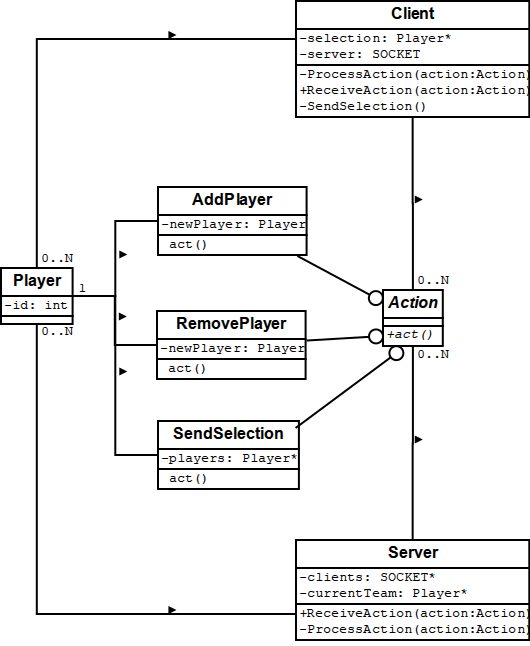
\includegraphics[scale=0.5]{Report01}
\caption{Class Diagram for UC 6 and 17 (Propose Team and Send Team Selection)}
\end{figure}

\begin{figure}[h]
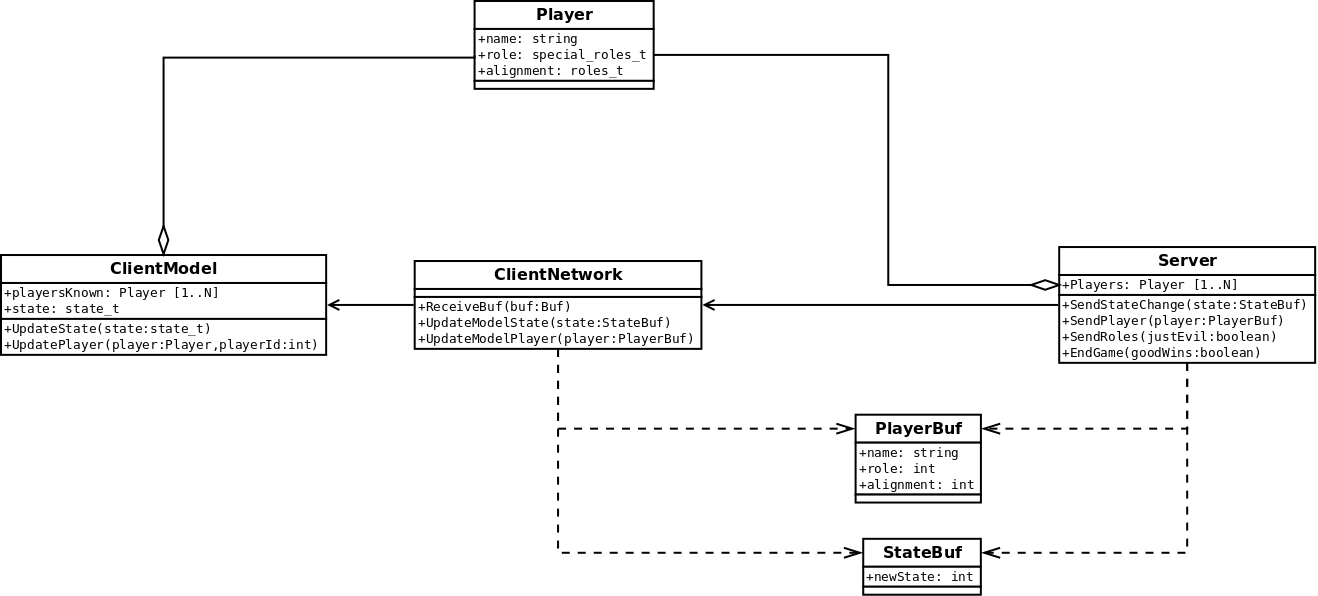
\includegraphics[scale=0.2]{Report02}
\caption{Figure 2: Class Diagram for UC 39 and 41 (Send Roles and Send Win/Loss)}
\end{figure}

\begin{figure}[h]
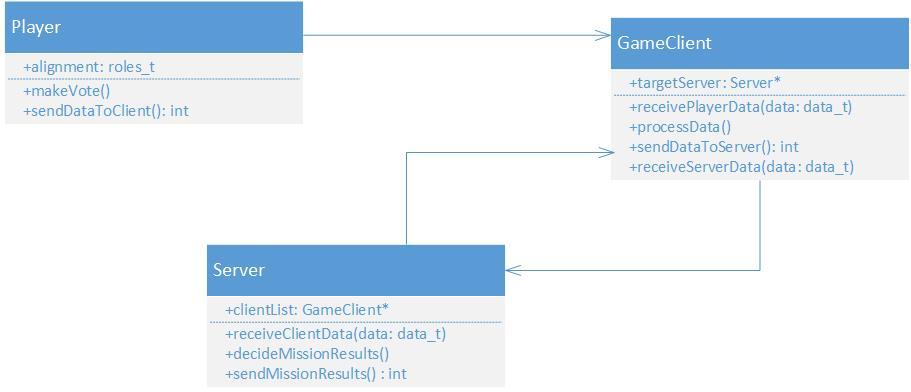
\includegraphics[scale=0.5]{Report03}
\caption{Class Diagram for UC 13 and 25 (Pass/Fail Mission and Send Mission Vote Results)}
\end{figure}
\end{center}

\pagebreak

\section{Future Plans}
\subsection{Ryan Kerr}
As one of the team leaders for this project, I realized during this project how difficult managing a group of people who are interested in a project can be, much less people who aren’t. Despite the fact that everyone was heavily invested in the project, it was very difficult to approximate the amount of work that should be assigned to each team. This meant that many iterations had the amount of work completed lopsided towards one group or another. I’m afraid this may have made our team less efficient than it could have been. Another thing I learned is how difficult it can be to break up work in a project that is incredibly connected.  Originally, Justin and I had planned on breaking work up into the “Client,” “Server,” and “GUI.” Unfortunately, this ended up being too difficult to reasonably complete, because the client and server were so heavily interconnected. Additionally, we regularly had a chicken-egg issue with GUI, since it was much easier to see what was going on in the client if the GUI was already completed, but it was very difficult to complete the GUI without the client. Outside of my management role in this group, I learned a lot about a model subscriber system, which is what we used to update the GUI whenever the client’s information changed. This made it very easy to abstract the GUI from the client, and allowed us to more easily split up work between groups. 

I believe that our group was very lucky to get team members who meshed together as well as we did. Justin and I did very little in the way of screening applicants, yet we somehow managed to get a diverse group of people. Thanks to this, our project went incredibly smoothly, since we had members who were very passionate about different areas of the codebase. The only downside to this approach is that I believe most of the team stayed in their comfort zone, rather than branching out and learning about new areas of coding. Everyone was able to, however, contribute heavily to the project, and focus on the coding process, as was intended in this class. Additionally, we were able to complete all of the use cases we had, and our final product is quite usable. Therefore, I believe this project was a great success, and I am glad to have worked with the rest of this group.
\subsection{Justin Koehler}
From my perspective, this project went shockingly well. Last semester in 427, my group worked together reasonably well, but we were typically behind on schedule and nobody was all that interested in getting work done. This semester, things came together much more reliably. As one of the team leaders, I was glad that we didn't have to expend a lot of effort on coercing the group to actually do its work. The biggest reason for this was clearly the degree of interest that we all held in the project itself. I personally may continue to develop Avalon Online in my spare time, simply because I find the project interesting enough to be worth it. That being said, there were a few issues during the development of the project. At the beginning of the semester, we had some difficulty in trying to design a component in a system that didn't exist yet, without making too much temporary work that would just be ripped out later. This also came up in later iterations, as Ryan and I would have to develop features "blind", as the GUI team were unable to easily do their part without our work already complete. These issues were relatively minor overall, though, and the personnel/management aspects were mostly smooth.

From a programming standpoint, I enjoyed the project immensely. The sections that Ryan and I handled (networking and game logic) allowed me to code to my strengths, as Ryan and I had both taken CS438 Networking previously, and I enjoy the kind of high-level system design that game logic programming entailed. One of the high points of the project was being able to depend on other teams to make usable components that I could easily interact with. Once Matt had fleshed out his design for the model, we were able to just use it with very little maintenance. In a similar vein, I have very little experience with UI design and writing GUI code, and so was not looking forward to completing those parts of the project. Being able to simply pass the data on to the GUI team, and then see the interface fully realized at the next meeting, was an exciting part of the work. In the end, we ended up completing the entire project as planned, and in a fairly solid manner, without the need for lots of ugly patches and hacks. Overall, the project is definitely a success.
\subsection{Matt Hoffman}
I’m very happy with how our project turned out. First of all, we finished all our goals which is saying something. We even had time to spare at the end allowing for polishing and stretch goals. This is in part because all of our team members had chemistry and were reliable. We were all able to meet up and discuss the state of our project and our goals rather candidly, keeping everyone up to date on what the others were working on. Also, when we divided up work everyone did their part quickly and kept the others in the loop. This allowed us to take complex tasks (like quest voting) and break them up into independent coding tasks and trust that everyone else would finish the requirements to make your code work. By breaking up into teams and leveraging each others’ work efficiently progress was much faster than most of my group projects and much less stressful.

Personally I was most responsible for the project architecture and middleware type code of our project. I worked with Mohammad to create the model and action queue systems which were what allowed the frontend GUI and the backend networking to communicate nicely. This framework took a lot of work upfront, but then shifted mostly to refactoring to add new features as the project developed. At that point I focused on improving the middleware by adding a few side features to the code (such as inheritable controller states allowing for simpler chat integration) and lua scripting for server configuration.
\subsection{Daniel Simpson}
On the whole, I think our project went very smoothly.  We hit our targets each iteration, and ended up with a good product.  The process reminded me of my internship from last summer, where I used a similar agile process with a similarly sized group.  This project went more smoothly than that one, due mostly to the group dynamic.  I think the biggest lesson I learned from this project is the importance of having a cohesive group with compatible members and good communication.

As I worked mostly on the UI, this project also impressed on me the difficulty and value of good user interface design.  Creating an ugly text-based interface is easy; a nice GUI takes significantly longer.  In fact, the amount of time management needed to produce a project even as small as this one surprised me.  For that, following a consistent design process was indispensable.    
\subsection{Jaime Roque}
Overall, I feel that this project is one of the most successful projects I’ve done to date in my college career. One of the major contributing factors to this is the team chemistry, as each of us had something to bring to the table whether it be experience in network programming or interface design. This not only allowed us to cover most of if not all of the requirements of our project, but it also allowed us to learn from each other as sub-groups interacted with the work done by other sub-groups. The team also made sure that everybody was up-to-date on the state of the project such that we did not move forward during the phase of a project until all team members were ready to do so. Contributing to the team chemistry, while not as important as other factors, are the similar interests shared amongst group members which facilitated friendly interactions. 

As one of the group members who worked on the GUI for our project, I have to say that it was an interesting experience not having to handle coding an extensive amount of back-end features. This reinforced the importance of abstraction and understanding the functionality of other people’s code as I had to go through the other sub-groups’ documentation in order to accomplish what I was assigned to do. As such, this also reinforced the importance of good documentation, especially when working in a large group where different members are working on different parts.
\subsection{Sachin Raghunathan}
I am extremely happy with our project. The best part was the way our subgroups worked. The decision that each subgroup specialized on distinct parts of the project and not changing the subgroup members for each week was genius. It meant that the requirements for each week (at least for the GUI team) became progressively easier. Even though this also meant that progress on one team depended on progress made by the other teams, I was happy to see that we worked in perfect synchronization to ensure that that happened. This was what allowed us to complete the requirements well in time for each week.

I worked on the GUI team with Daniel and Jaimie. There was a slight learning curve at the start in working with qt, but like i said, it got progressively easier as we gained familiarity with it. I thought that we did a pretty good job with the GUI considering we had quite some information to display. In general, I think the game works quite well and while it could obviously use improvements, it provides an entertaining (and unique) avalon experience.
\subsection{Mohammed Askari}
Overall, I think that the project went very well. We managed to finish all of our use cases and user stories by the final iteration without ever having to rush to get tasks done at the last minute. Our group had very good chemistry, which made group meetings much less of a chore, even though they might have taken a little longer from all of our small talk. Our process of splitting into subgroups to work on specific parts of the code was terrific for this project. Matt and I were responsible for the Model part of the MVC architecture and integrating actions, which flow throughout our project. The backend work was split fairly evenly between our subgroup and Ryan and Justin and we spent time at group meetings mostly trying to connect our portions with theirs and/or the GUI. It was a pleasant surprise that almost everything was done in a quality and timely fashion by every subgroup.

The most important thing that I learned from this project is the value of team chemistry. Compared to last semester, when there were times that my subgroup was the only one to have our part ready by the agreed upon time, this group was a lot more responsible at every point. Part of this is because working together with this group was enjoyable and there was a positive atmosphere. I also learned about proper planning and setting reasonable goals and deadlines. Planning ahead can be just as important as the coding itself since it gives everyone a firm measure of what they need to get done and how long they have to do it, without making it seem like an impossible task.
\end{document}